\chapter{Pruebas} \label{pruebas}

{\color{blue}

Para realizar las pruebas, he tenido la oportunidad de usar una Raspberry PI \cite{raspberry-specs}. De esta manera he podido hacer uso de las funcionalidades de este dispositivo para mostrar de una manera más realista el potencial de la aplicación y también de explotar una vulnerabilidad.

\section{Conectar un cliente}

Tal y como vimos en \ref{connect-dispositivo}, una vez ya hemos creado nuestro primer endpoint, podemos conectar un cliente y obtener y enviar algunos metadatos. Como se analizó \ref{eleccion-framework}, Kaa IoT es un framework que soporta varios protocolos donde nos encontramos con HTTP y MQTT \ref{protocolos}.

Para hacer uso de los protocolos y completar la integración del cliente necesitaremos el nombre de la versión y el token del endpoint. En esta sección se va a mostrar como hacer uso de ambos protocolos, concretamente de las órdenes para poder ejecutar la conexión con nuestro dispositivo, en la sección de \textit{Pruebas} \ref{pruebas} se mostrarán los datos que obtenemos tras su ejecución.\\

\subsection{Conexión mediante HTTP} \label{http-connection}

Para obtener todos los atributos de los metadatos con \textbf{HTTP} vamos a hacer uso de cURL \footnote{Es un proyecto de software consistente en una biblioteca y un intérprete de comandos orientado a la transferencia de archivos. Soporta los protocolos FTP, FTPS, HTTP, HTTPS, TFTP, SCP, SFTP, Telnet, DICT, FILE y LDAP, entre otros.} para enviar una solicitud de actualización de datos del dispositivo.

\begin{lstlisting}[language=bash]
curl - -location - -request POST 'https://connect.cloud.kaaiot.com:443/kp1/
<app-version-name>/epmx/<endpoint-token>/update/keys' \
- -data-raw '{
    "model": "Raspberry PI",
    "mac": "00-14-22-01-23-45"
}'
\end{lstlisting}

Ejecutando esta instrucción añadiremos nuevos metadatos a nuestro dispositivo, concretamente la dirección física y el modelo de este.

\subsection{Conexión mediante MQTT} \label{mqtt-connection}

Para hacer la conexión mediante \textbf{MQTT} se ha optado por la opción de usar Python en su versión 3.10, obtenemos un código como el siguiente.

\begin{lstlisting}[language=Python]
import itertools
import json
import queue
import sys
from subprocess import Popen, PIPE


class MetadataClient:

    def __init__(self, client, app_version, endpoint_token):
        self.client = client
        self.app_version = app_version
        self.endpoint_token = endpoint_token
        self.metadata_by_request_id = {}
        self.global_request_id = itertools.count()
        get_metadata_subscribe_topic = f'kp1/{self.app_version}/epmx/{self.endpoint_token}/get/#'
        self.client.message_callback_add(get_metadata_subscribe_topic, self.handle_metadata)

    def handle_metadata(self, client, userdata, message):
        request_id = int(message.topic.split('/')[-2])
        if message.topic.split('/')[-1] == 'status' and request_id in self.metadata_by_request_id:
            print(f'<--- Received metadata response on topic {message.topic}')
            metadata_queue = self.metadata_by_request_id[request_id]
            metadata_queue.put_nowait(message.payload)
        else:
            print(
                f'<--- Received bad metadata response on topic {message.topic}:\n{str(message.payload.decode("utf-8"))}')

    def get_metadata(self):
        request_id = next(self.global_request_id)
        get_metadata_publish_topic = f'kp1/{self.app_version}/epmx/{self.endpoint_token}/get/{request_id}'

        metadata_queue = queue.Queue()
        self.metadata_by_request_id[request_id] = metadata_queue

        print(f'---> Requesting metadata by topic {get_metadata_publish_topic}')
        self.client.publish(topic=get_metadata_publish_topic, payload=json.dumps({}))
        try:
            metadata = metadata_queue.get(True, 5)
            del self.metadata_by_request_id[request_id]
            return str(metadata.decode("utf-8"))
        except queue.Empty:
            print('Timed out waiting for metadata response from server')
            sys.exit()

    def patch_metadata_unconfirmed(self, metadata):
        partial_metadata_update_publish_topic = f'kp1/{self.app_version}/epmx/{self.endpoint_token}/update/keys'

        print(f'---> Reporting metadata on topic {partial_metadata_update_publish_topic}\nwith payload {metadata}')
        self.client.publish(topic=partial_metadata_update_publish_topic, payload=metadata)

    def hardware_devices(self):
        return Popen(['lsusb'], stdout=PIPE, encoding='utf-8').communicate()[0]

    def set_metadata(self):
        metadata_to_report = json.dumps(
            {"model": "Raspberry PI",
             "mac": "b8-27-eb-f8-00-af",
             "devices": self.hardware_devices()
             }
        )
        return metadata_to_report

\end{lstlisting}

La ejecución de este código produce un efecto similar que el visto con HTTP. En este caso se ha creado una clase \textit{MetadataClient}, su objetivo es el de actualizar los metadatos del dispositivo en nuestra aplicación. Cada vez que se establece la conexión se analiza los dispositivos conectados a la Raspberry y se envían a la aplicación (como ejecutar en la terminal de linux, lusb).


\begin{figure}[p]
    \centering
    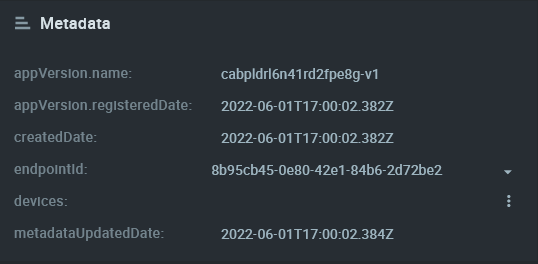
\includegraphics[width=\linewidth]{imagenes/metadata-old.png}
    \caption{Metadatos una vez creada nuestra aplicación}
    \label{fig:figure11}
\end{figure}


\section{Recogida de datos y ejecución de comandos de un dispositivo}


\subsection{Envio de datos mediante MQTT}

Al igual que en la sección \ref{mqtt-connection} tenemos un código para hacer el envió de datos y la ejecución de comandos, para ello definimos dos endpoints, uno para encender un led y el otro para apagar un led.


El código es el siguiente:

\begin{lstlisting}[language=Python]
import json
import signal
import time

from gpiozero import LED, CPUTemperature


def temp_data():
    cpu = CPUTemperature()
    return cpu.temperature


class KaaClient:

    def __init__(self, client, app_version, endpoint_token, host, port):
        self.client = client
        self.app_version = app_version
        self.endpoint_token = endpoint_token
        self.host = host
        self.port = port
        self.metadata_update_topic = f'kp1/{self.app_version}/epmx/{self.endpoint_token}/update/keys'
        self.data_collection_topic = f'kp1/{self.app_version}/dcx/{self.endpoint_token}/json'

        self.led = LED(17)

        command_turn_on_topic = f'kp1/{self.app_version}/cex/{self.endpoint_token}/command/turnon/status'
        self.client.message_callback_add(command_turn_on_topic, self.handle_turn_on_command)
        self.command_turn_on_result_topik = f'kp1/{self.app_version}/cex/{self.endpoint_token}/result/turnon'

        command_turn_off_topic = f'kp1/{self.app_version}/cex/{self.endpoint_token}/command/turnoff/status'
        self.client.message_callback_add(command_turn_off_topic, self.handle_turn_off_command)
        self.command_turn_off_result_topik = f'kp1/{self.app_version}/cex/{self.endpoint_token}/result/turnoff'

    def connect_to_server(self):
        print(
            f'Connecting to Kaa server at {self.host}:{self.port} using application version {self.app_version}'
            f' and endpoint token {self.endpoint_token}')
        self.client.connect(self.host, self.port, 60)
        print('Successfully connected')

    def disconnect_from_server(self):
        print(f'Disconnecting from Kaa server at {self.host}:{self.port}...')
        self.client.loop_stop()
        self.client.disconnect()
        print('Successfully disconnected')

    def compose_data_sample(self):
        return json.dumps([
            {
                "timestamp": int(round(time.time() * 1000)),
                "temperature": int(temp_data())
            }
        ])

    def on_message(client, userdata, message):
        print(f'<-- Received message on topic "{message.topic}":\n{str(message.payload.decode("utf-8"))}')

    def handle_turn_on_command(self, client, userdata, message):
        print(f'<--- Received "turn on" command on topic {message.topic} \nTurning on...')
        self.led.on()
        command_result = self.compose_command_result_payload(message)
        print(f'command result {command_result}')
        client.publish(topic=self.command_turn_on_result_topik, payload=command_result)
        # With below approach we don't receive the command confirmation on the server side.
        # self.client.disconnect()
        # time.sleep(5)  # Simulate the reboot
        # self.connect_to_server()

    def handle_turn_off_command(self, client, userdata, message):
        print(f'<--- Received "turn on" command on topic {message.topic} \nTurning off...')
        self.led.off()
        command_result = self.compose_command_result_payload(message)
        print(f'command result {command_result}')
        client.publish(topic=self.command_turn_on_result_topik, payload=command_result)

    def compose_command_result_payload(self, message):
        command_payload = json.loads(str(message.payload.decode("utf-8")))
        print(f'command payload: {command_payload}')
        command_result_list = []
        for command in command_payload:
            commandResult = {"id": command['id'], "statusCode": 200, "reasonPhrase": "OK", "payload": "Success"}
            command_result_list.append(commandResult)
        return json.dumps(
            command_result_list
        )


class SignalListener:
    keepRunning = True

    def __init__(self):
        signal.signal(signal.SIGINT, self.stop)
        signal.signal(signal.SIGTERM, self.stop)

    def stop(self, signum, frame):
        print('Shutting down...')
        self.keepRunning = False

\end{lstlisting}

Con este código se entra en un bucle donde se van haciendo llamadas al dispositivo y recogiendo información. La información que nos llega viene en formato JSON. Se usa la librería \textit{gpiozero} para encender/apagar el led y obtener la temperatura de la CPU. 

También se ha creado un fichero para cargar la configuración necesaria (endpoint ID, host, puerto) y ejecutar el programa.

\begin{lstlisting}[language=Python]

import random
import string
import time

from metadataClient import MetadataClient
from kaaClient import KaaClient
from kaaClient import SignalListener

import paho.mqtt.client as mqtt
from decouple import config

KPC_HOST = config('KPC_HOST', cast=str)
KPC_PORT = config('KPC_PORT', cast=int)

APPLICATION_VERSION = config('APPLICATION_VERSION', cast=str)
ENDPOINT_TOKEN = config('ENDPOINT_TOKEN', cast=str)


def main():
    # Iniciar la conexion con el servidor
    print(
        f'Connecting to Kaa server at {KPC_HOST}:{KPC_PORT} using application version {APPLICATION_VERSION}'
        f' and endpoint token {ENDPOINT_TOKEN}')

    client_id = ''.join(random.choice(string.ascii_uppercase + string.digits) for _ in range(6))
    client = mqtt.Client(client_id=client_id)
    client.connect(KPC_HOST, KPC_PORT, 60)
    client.loop_start()

    metadata_client = MetadataClient(client, APPLICATION_VERSION, ENDPOINT_TOKEN)

    # Obtener los atributos de los metadatos del endpoint actual
    retrieved_metadata = metadata_client.get_metadata()
    print(f'Retrieved metadata from server: {retrieved_metadata}')

    # Actualizar parcialmente los metadatos del endpoint
    metadata_to_report = metadata_client.set_metadata()
    metadata_client.patch_metadata_unconfirmed(metadata_to_report)

    time.sleep(5)
    client.disconnect()

    # Initiate server connection
    client = mqtt.Client(client_id=''.join(random.choice(string.ascii_uppercase + string.digits) for _ in range(6)))

    data_collection_client = KaaClient(client, APPLICATION_VERSION, ENDPOINT_TOKEN, KPC_HOST, KPC_PORT)
    data_collection_client.connect_to_server()

    client.on_message = data_collection_client.on_message

    # Start the loop
    client.loop_start()

    # Send data samples in loop
    listener = SignalListener()
    while listener.keepRunning:

        payload = data_collection_client.compose_data_sample()

        result = data_collection_client.client.publish(topic=data_collection_client.data_collection_topic,
                                                       payload=payload)
        if result.rc != 0:
            print('Server connection lost, attempting to reconnect')
            data_collection_client.connect_to_server()
        else:
            print(f'--> Sent message on topic "{data_collection_client.data_collection_topic}":\n{payload}')

        time.sleep(3)

    data_collection_client.disconnect_from_server()


if __name__ == '__main__':
    main()


\end{lstlisting}

Se usa \textit{decouple} para evitar mostrar los datos de configuración de la aplicación, usando un fichero \textit{.env}.

Se muestra a continuación pruebas de la ejecución del código.


\begin{figure}[p]
    \centering
    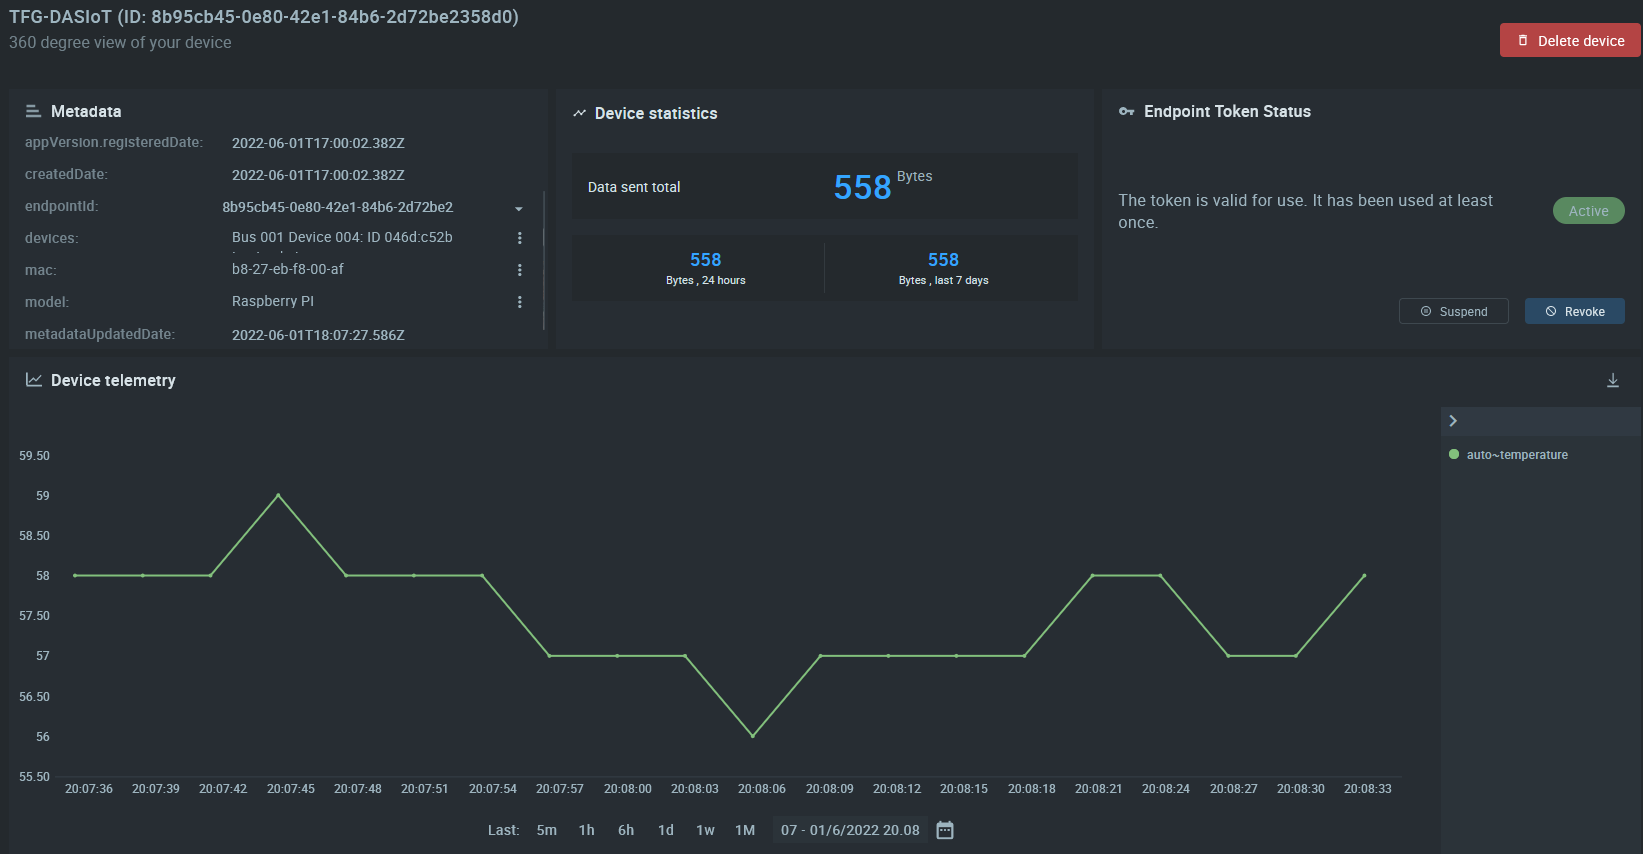
\includegraphics[width=\linewidth]{imagenes/data-execution.png}
    \caption{Metadatos actualizados y telemetría de la temperatura de la CPU}
    \label{fig:figure13}
\end{figure}

\begin{figure}[p]
    \centering
    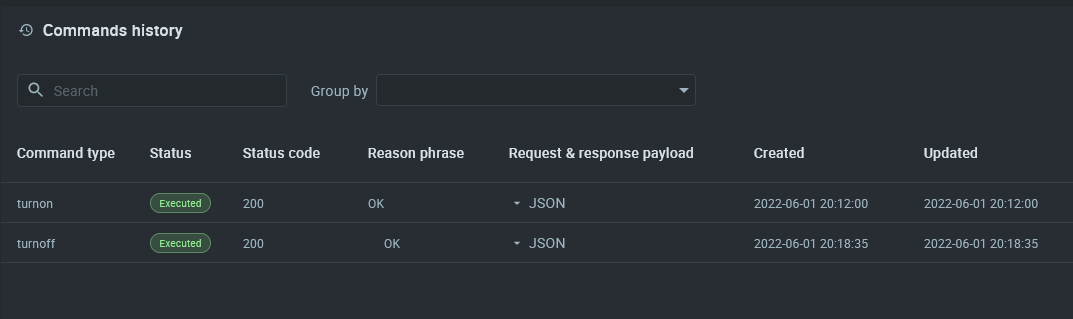
\includegraphics[width=\linewidth]{imagenes/command-execution.png}
    \caption{Encendido y apagado del led}
    \label{fig:figure14}
\end{figure}

\begin{figure}[p]
    \centering
    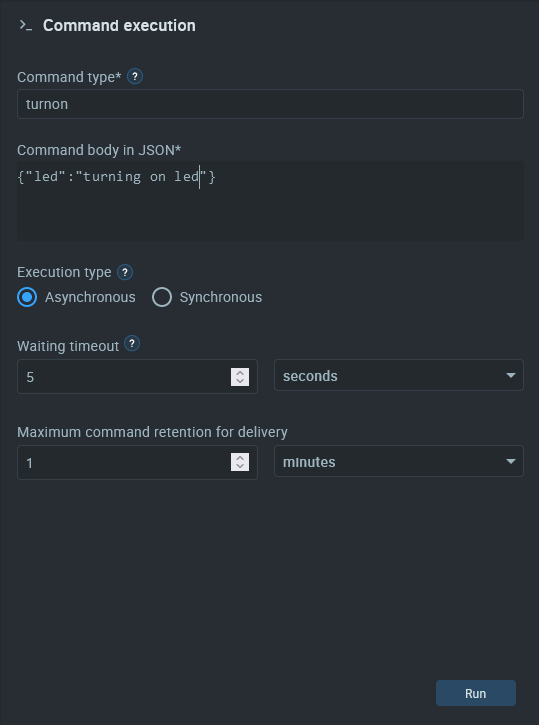
\includegraphics[width=\linewidth]{imagenes/turn-on-led.png}
    \caption{Petición de encendido del led}
    \label{fig:figure15}
\end{figure}

\begin{figure}[p]
    \centering
    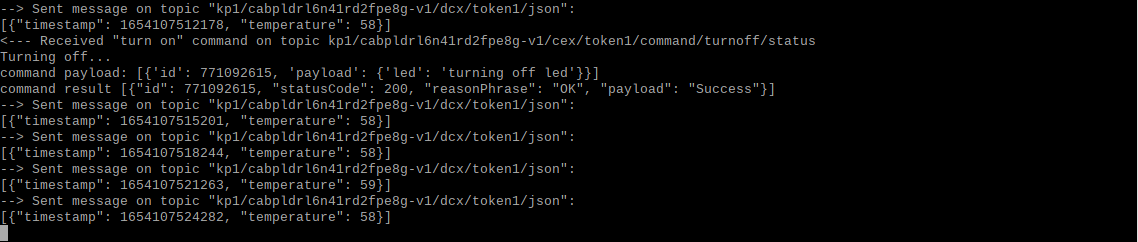
\includegraphics[width=\linewidth]{imagenes/2022-06-01-201846_1920x1080_scrot.png}
    \caption{Inicio de conexión y envio de datos a la aplicación}
    \label{fig:figure16}
\end{figure}

\begin{figure}[p]
    \centering
    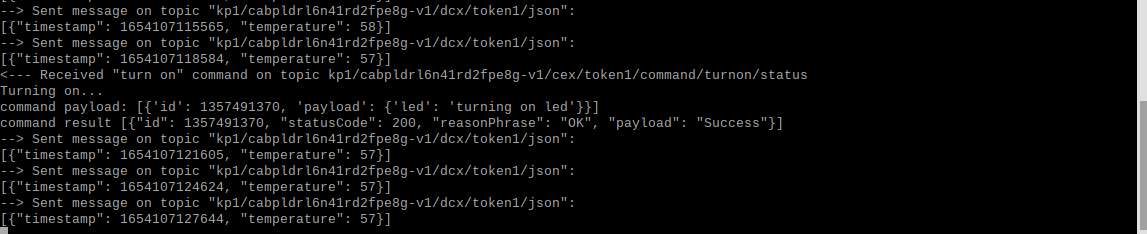
\includegraphics[width=\linewidth]{imagenes/2022-06-01-201209_1920x1080_scrot.png}
    \caption{Encendiendo el led}
    \label{fig:figure17}
\end{figure}

\begin{figure}[p]
    \centering
    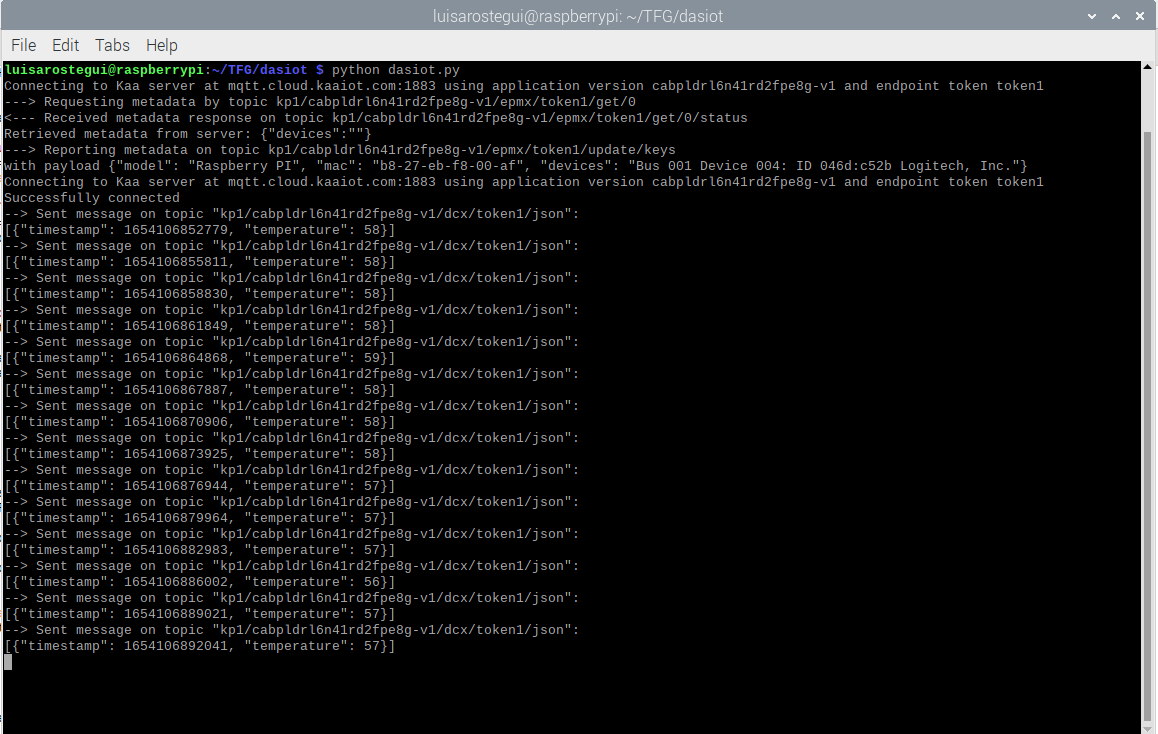
\includegraphics[width=\linewidth]{imagenes/2022-06-01-200813_1920x1080_scrot.png}
    \caption{Apagando el led}
    \label{fig:figure18}
\end{figure}



}